\chapter{Model neuron as Point neurons}
\label{chap:point-neuron}

{\bf What make the brain so difficulty to understand?}:
\begin{itemize}
\item large number of cells, with different shapes and electrical
  properties
   
\item bewildering connection patterns between neurons in a region and between
hundreds of nuclear regions (Sect.\ref{sec:nuclei_structure}).

\item dozens of neurotransmitters and modulators exist, each with its
  own repertoire of receptors and synaptic actions.
  
   
\item current available techniques allow access to only a few cells,
  while a comprehensive approach requires measuring hundreds of them.
\end{itemize}

So, a neuron receives the input signals via its many synapses on the dendrites
(Sect.\ref{sec:synapse-number-per-neuron}). The inputs, in the form of membrane
depolarization (for excitatory input) or membrane hyperpolarization (for
inhibitory input) come from the active synapses located at different places on
the neuron's dendrite. Sect.\ref{sec:nerve-cells} helps us to understand the
roles of these different neuron components.
Depending on the value of the summation of all input at the soma (or axon
hillock) - the spike initiation site, the membrane of the neuron's soma can be
in either {\bf electrotonus} or {\bf transient} behavior -
Sect.\ref{sec:electrotonus_vs_transient}.
The cell is in transient behavior, i.e. an AP in the form of a spike is
generated - typically it is not a single spike but can be a sequence of spikes
forming a bursting behavior- Sect.\ref{sec:bursts},
Sect.\ref{sec:burst_cluster}.

\begin{mdframed}

{\bf Neuron R15} is the first intrinsically bursting neuron to receive
extensive study. R15 is found in abdominal ganglion of the gastropod mullusc {\it Aplysia
Carlifornica}\footnote{\url{http://www.scholarpedia.org/article/Aplysia_R15_neuron}}.

Thank to the well organized of neurons in hippocampus into
layers; hippocampus has frequently been used as a model system for studying
neurophysiology. With hippocampus, the flow of information is largely
unidirectional. (Sect.\ref{sec:signal_hippocampus_cell}).

\end{mdframed}  


% To build a broader range of knowledge in studying neurons, in this chapter, we
% will first introduce different types of neurons (Sect.\ref{sec:neuron-types}),
% and then cable theory to describe AP propagation (Sect.\ref{sec:model-cell}).
\textcolor{red}{One of the unique characteristics of neurons is the constant AP
shape in the form of {\bf spike} regardless of the locations and neuron types}.
Early models focus on to build the model that can reprelicate the spiking
behavior, e.g.
individual spike, or bursting (Sect.\ref{sec:bursting_behavior})).

The models are classified into conductance-based models ($V_m$ and a series
of ionic conductance $g_i$) and current-based models ($V_m$ and a series of
ionic current $I_i$). 
\begin{itemize}
  \item conductance-based models: Hodgkin-Huxley models \ldots
  
  \item current-based models: point neurons (e.g. integrate-and-fire models),
  \ldots
\end{itemize}

In terms of number of state variables:
\begin{itemize}
  \item n-D models: the many state variables are used, and all of them are in
  linear terms
  
  The most popular one is Hodgkin-Huxley model (conductance-based model)
  (Sect.\ref{sec:Hodgkin-Huxley-1952-model}) which is a phenomenological model but
  also incorporate different ion channels. 

  \item 1-D model:
The crudest models tried to characterize the neuron behavior by one variable,
usually thought of as the transmembrane voltage.

Example: RC leaky integrator: Sect.\ref{sec:RC-leaky}
  
  \item 2-D models: in order to capture the many observed firing patterns, and
  keep the number of state variables small, it usually requires the introduction
  of nonlinearities (Izhikevich, 2003; Brette \& Gerstner, 2005; Touboul, 2008).

Example: the reduced model of FitzHugh-Nagumo using two
variables (Sect.\ref{sec:fitzh-nagumo-model}) with the goal to simplify the
computational demand, but to focus on the general shape of AP.
Others: Morris-Lecar, and Izhikevich models (Sect.\ref{sec:Izhikevich-2003})
  

\end{itemize}

\begin{figure}[htb]
  \centerline{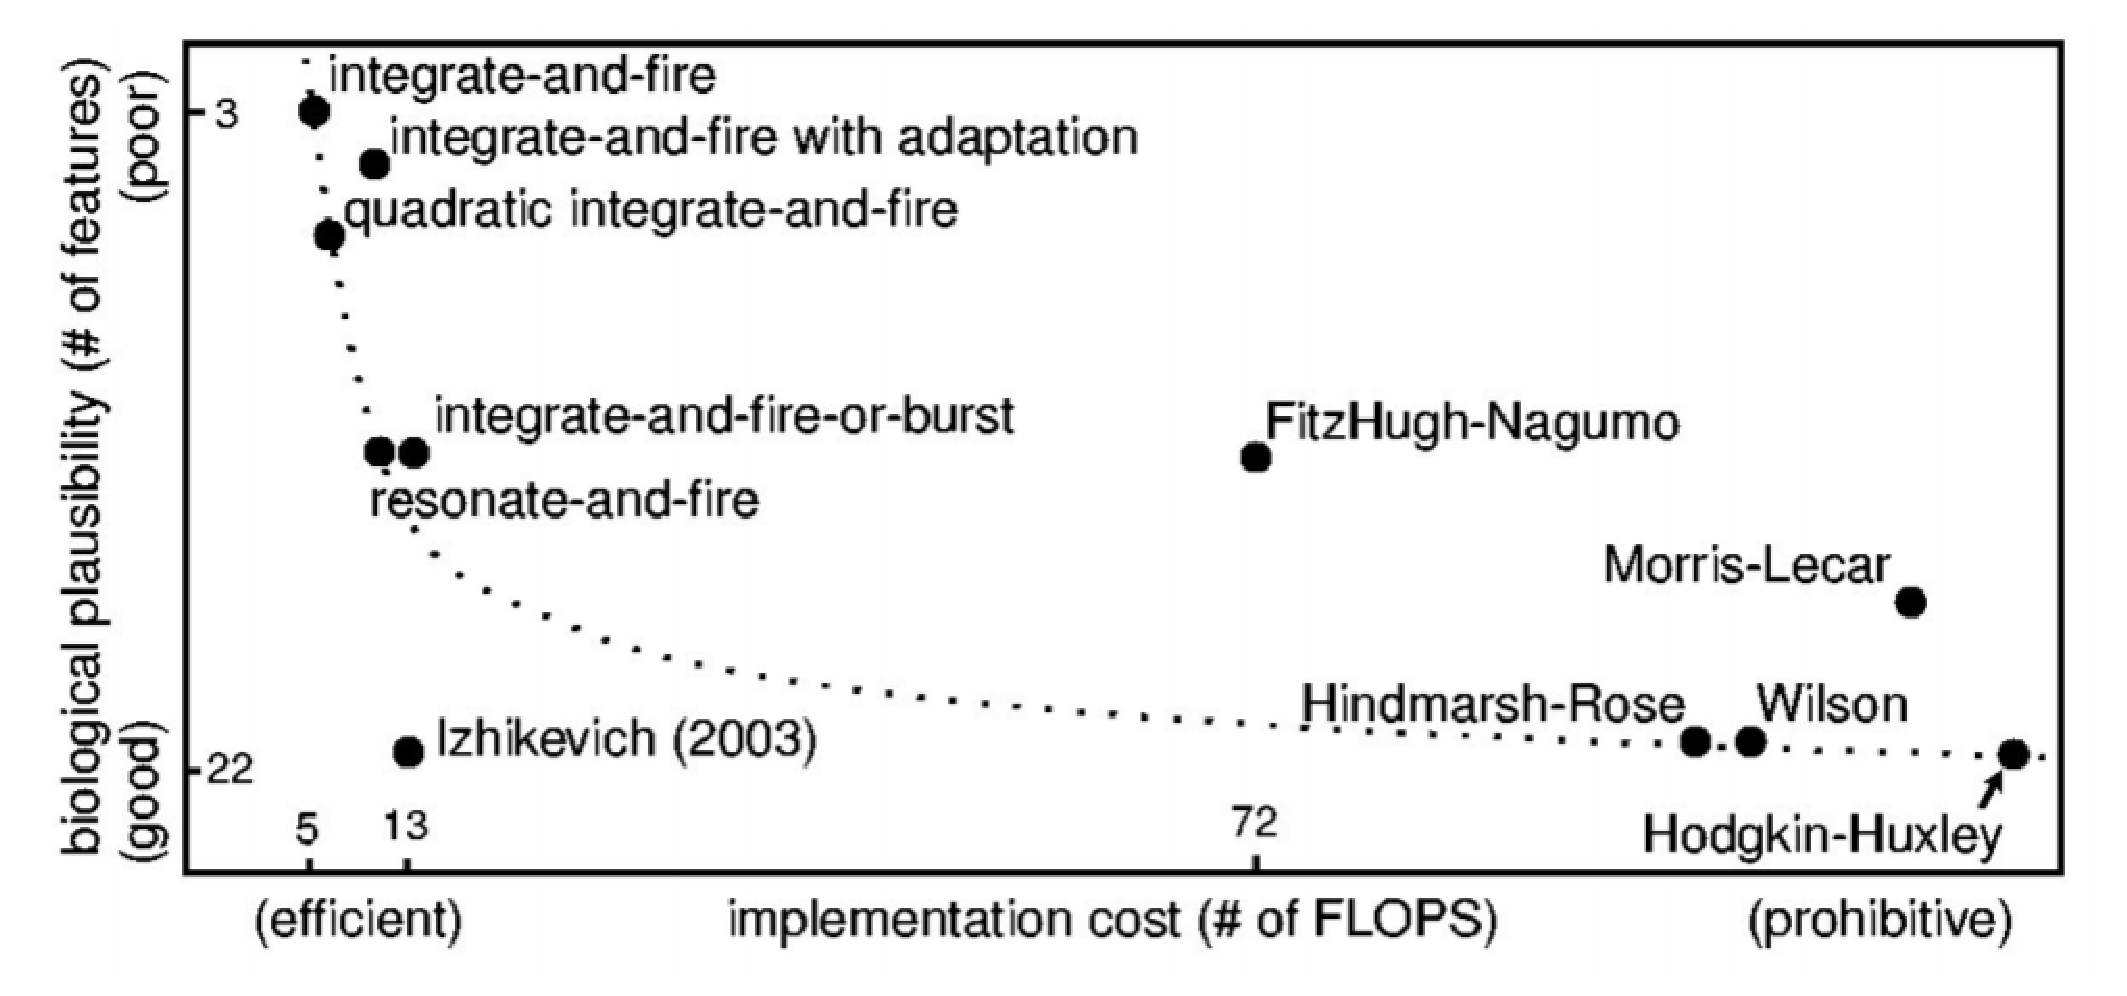
\includegraphics[height=5cm]{./images/compare-models.eps}}
  \caption{Comparison of models }\label{fig:compare-models}
\end{figure}


\section[Point neuron: leaky integrate-and-fire (electrotonic phase))]{Leaky
Integrate-and-Fire model (LIF neuron, RC leaky integrator, spherical shell, point neuron)}
\label{sec:leaky_integrate-and-fire_model}
\label{sec:RC-leaky}
\label{sec:point-neuron}

The leaky integrate-and-fire (LIF) neuron is probably one of the simplest
spiking neuron models, Fig.\ref{fig:compare-models}, but it is still very
popular due to the ease with which it can be analyzed and simulated.
\textcolor{red}{The integrate-and-fire neuron model is {\bf a point neuron}
(single compartment) model in which the spatial structure of the neuron
associated with the dendrites is neglected, and the state of the neuron is
characterized by its membrane potential $V_m(t)$}.



\subsection{Assumption: spherical cell}
\label{sec:spherical-cell}

ASSUMPTIONS:
\begin{enumerate}
  \item point neurons (isopotential), i.e. no spatial effect
  
  \item ignore transient phase

As the unique feature of constant spike shape among neurons, early models ignore
the dynamics of the cells at transient phase - and only focus
on the behavior of the neuron at the electrotonic phase, i.e. how the neuron's membrane changes
that can lead to (or failt to lead to) the spike. A spike is created if the
membrane potential passes a given threshold.

Suppose we have a spherical cell with diameter $d$, injected with a current
$I_\app$(t) directly into the intracellular of the cell.
Assuming the cell has passive membrane behavior. As shown in
Fig.\ref{fig:spherical-cell-passive-membrane}, we can assume iso-potential (i.e.
neglect any spatial dependencies). The cell membrane can be conceptualized as
being made up from many small RC circuits.

\textcolor{red}{In the simplest form} (Lapique 1907) with iso-potential
assumption, the cell can be reduced to a single RC compartment in series with a
current source $I_\app$. The membrane capacitor is charged until it reaches the
threshold for producing an AP (a spike), and the potential is reset.
In the model, if $V_m$ reaches the threshold from below (i.e. it reaches the
transient phase with very stiff behavior and may requires very small time-step
to calculate), the model is reset after it pass the slow time-scale, i.e.
passing the threshold $V_\th$. So, the model separates the two different
time-scale (1. relatively slow subthreshold integration, 2. vary rapid spike
generation), by focusing only on the slow time-scale.


\begin{figure}[htbp]
\centerline{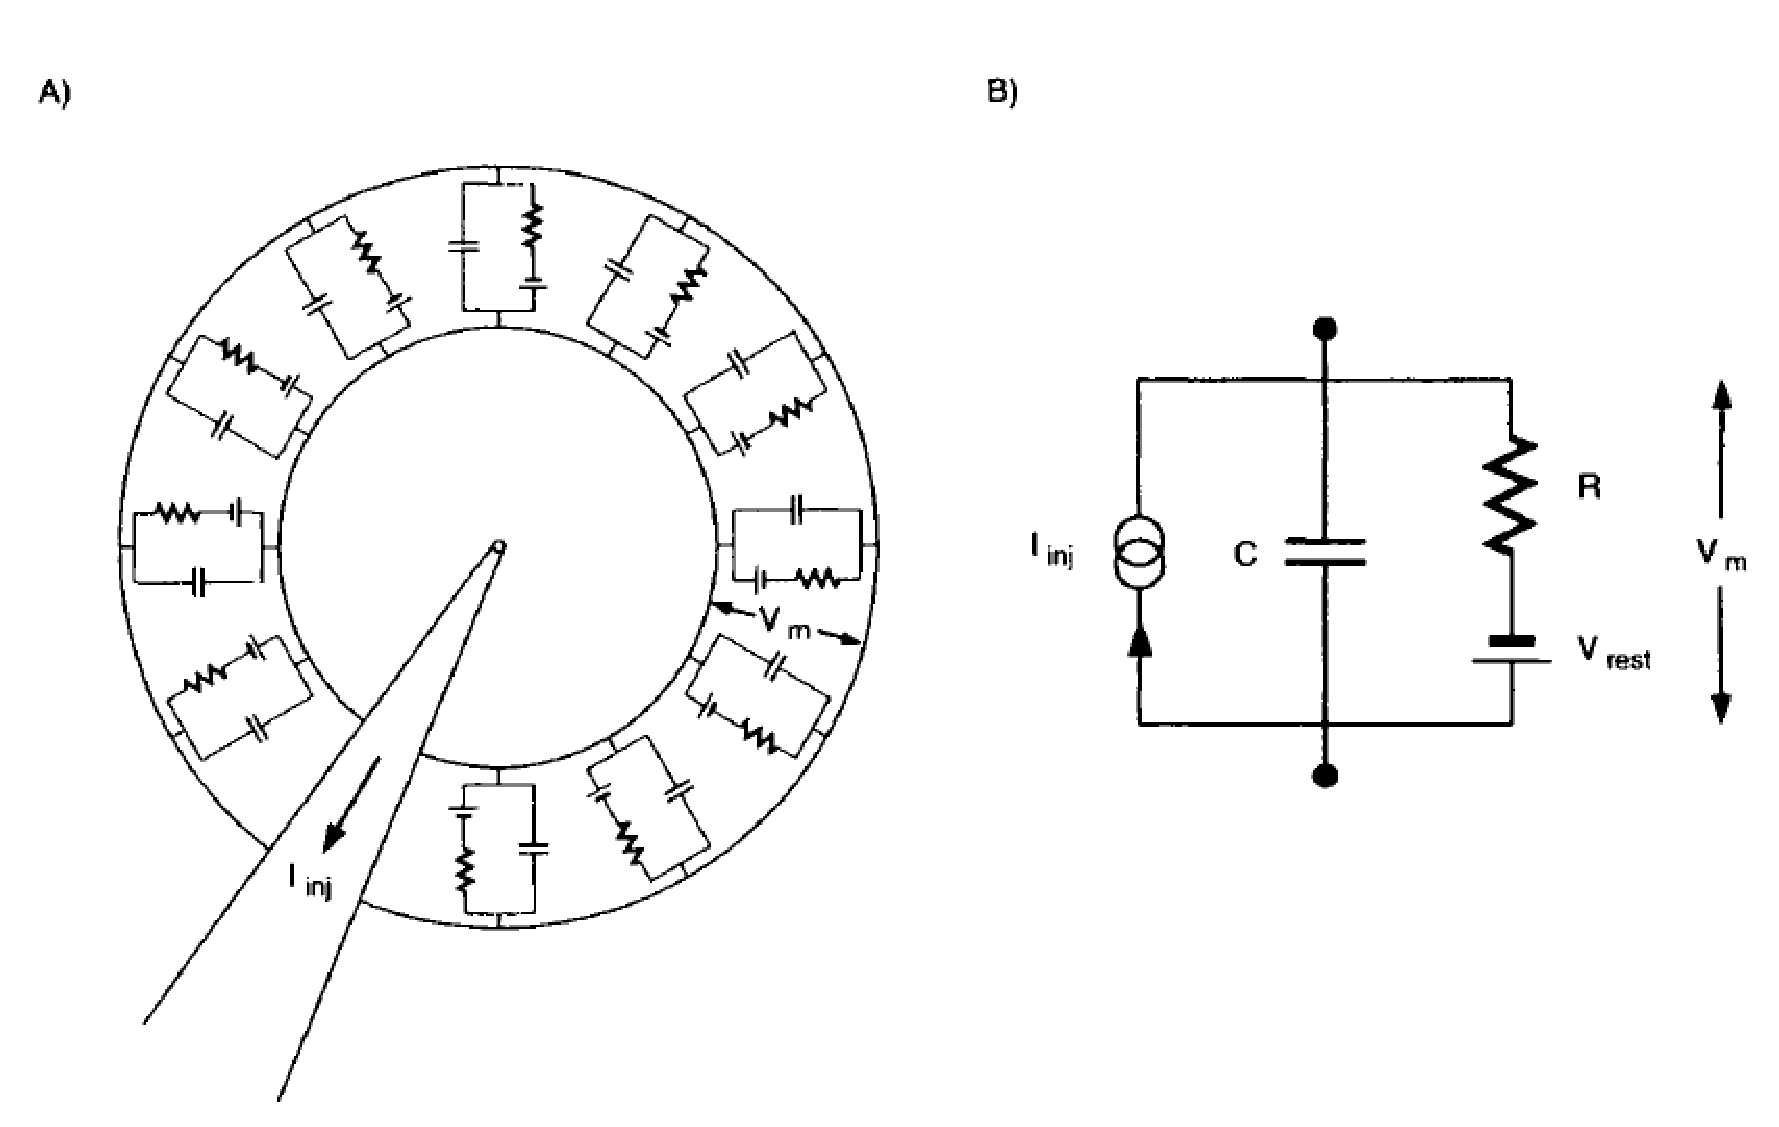
\includegraphics[height=6cm]{./images/spherical-cell-passive-membrane.eps}}
\caption{(A) A spherical cell of isopotential with passive membrane injected
with a current $I_\app$; (B) The equivalent electrical RC circuit in parallel
with an ideal current source $I_\app$}
\label{fig:spherical-cell-passive-membrane}
\end{figure} 



NOTE: Here, the spiking events are not explicitly modelled until
Sect.\ref{sec:Integrate-and-Fire-Spike}.

   \item artificially model the absolute refractory period: the neuron has a
   certain time period after the spike that it cannot trigger a new spike

The mechanism is not modelled. Instead, \textcolor{red}{to artificially
incorporate the absolute refractory period} $\Delta_{abs}=\tau_r$, i.e. the time
during which there can not be another spike, immediately after $V(t)$ hit
$V_\th$, we just clamp $V(t)$ to $V_r$ during that time, and the leaky
integration process is re-calculated following that delay $\Delta_{abs}$ after
the spike.
   
\end{enumerate}


A cell, e.g. the neuron, is assumed the spherical shape with surface membrane
area $A=4\pi a^2$ (cm$^2$).
In the simplest form, the cell is modelled as a single lumped-RC, with R in
parallel with a capacitor C.
\begin{eqnarray}
  \label{eq:493}
  \R &=& \frac{\Rm}{A} \\
  \C &=& \Csc A
\end{eqnarray}
with $\Rm$ is membrane resistivity across a unit area (or specific
membrane resistance) (Ohm.cm$^2$), and $\Csc$ is specific membrane capacitance
(i.e. capacitance per a unit area) ($\mu$F/cm$^2$). R ($\Omega$) and C ($\mu$F)
are the total membrane resistance and total membrane capacitance, respectively, for the cell.

\begin{figure}[hbt]
  \centerline{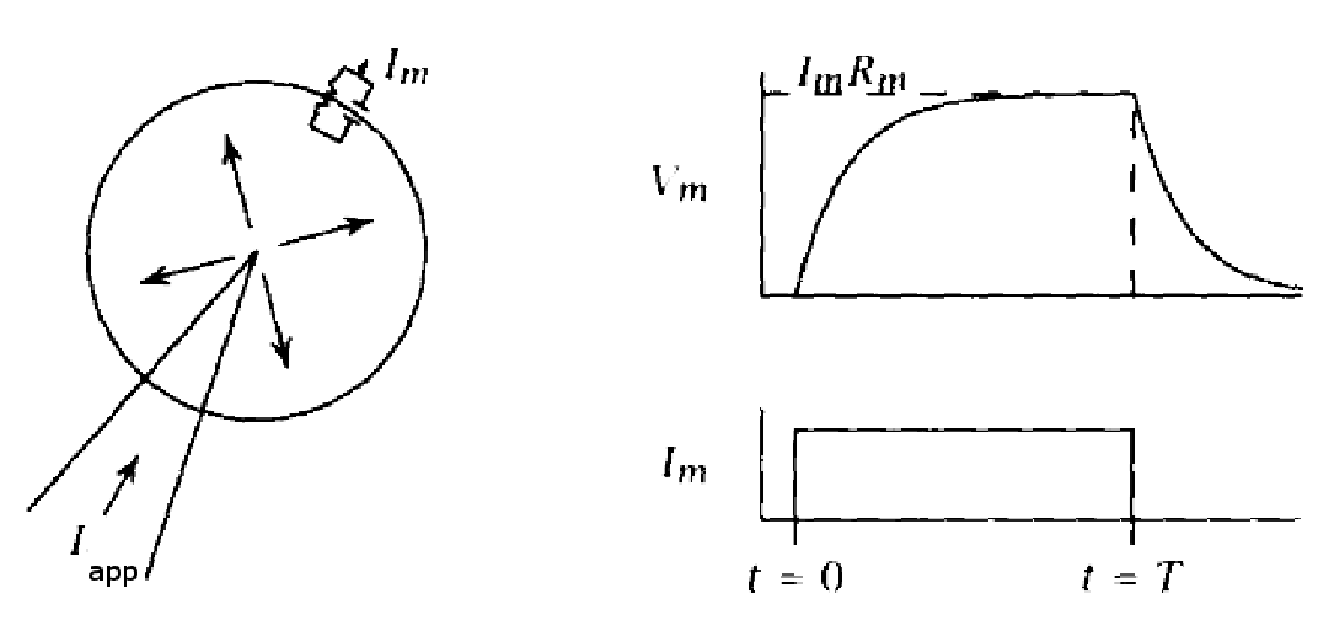
\includegraphics[height=3.8cm,
    angle=0]{./images/sphere_cell.eps}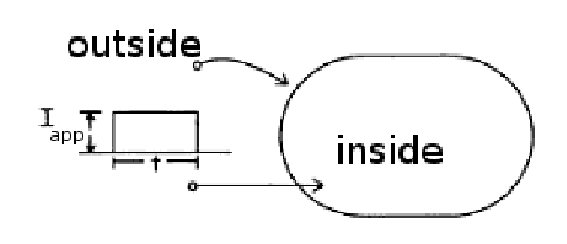
\includegraphics[height=1.7cm,
    angle=0]{./images/step_current.eps} }
\caption{Injection of a step current  $I_\app $ to an isopotential cell.}
\label{fig:sphere_cell}
\end{figure}

\begin{framed}
This is the simplest representation of a cell - which can fit modeling to the
neuron's soma. It's a sphere with the \textcolor{red}{essential assumption of
membrane potential of isopotential} for the whole cell membrane surface (intracellular +
extracellular). Thus, injected current through such cell $I_\app $ would be
uniformly distributed across the surface of the cell; and all membrane
components are electrically in parallel. Thus, the response of any patch will be
the same as any other patches. The entire surface membranes behaves
synchronously like a single macroscopic patch~\citep{plonsey2000bqa}.

{\bf NOTE}: Here, the notation $v$ is used rather than $V_m$ since the quantity
of interest is the change in the transmembrane potential relative to its
baseline $v=V_m-E_r$.
\end{framed}


\subsection{Model formula}
\label{sec:LIF-formula}

\begin{figure}[htb]
\centerline{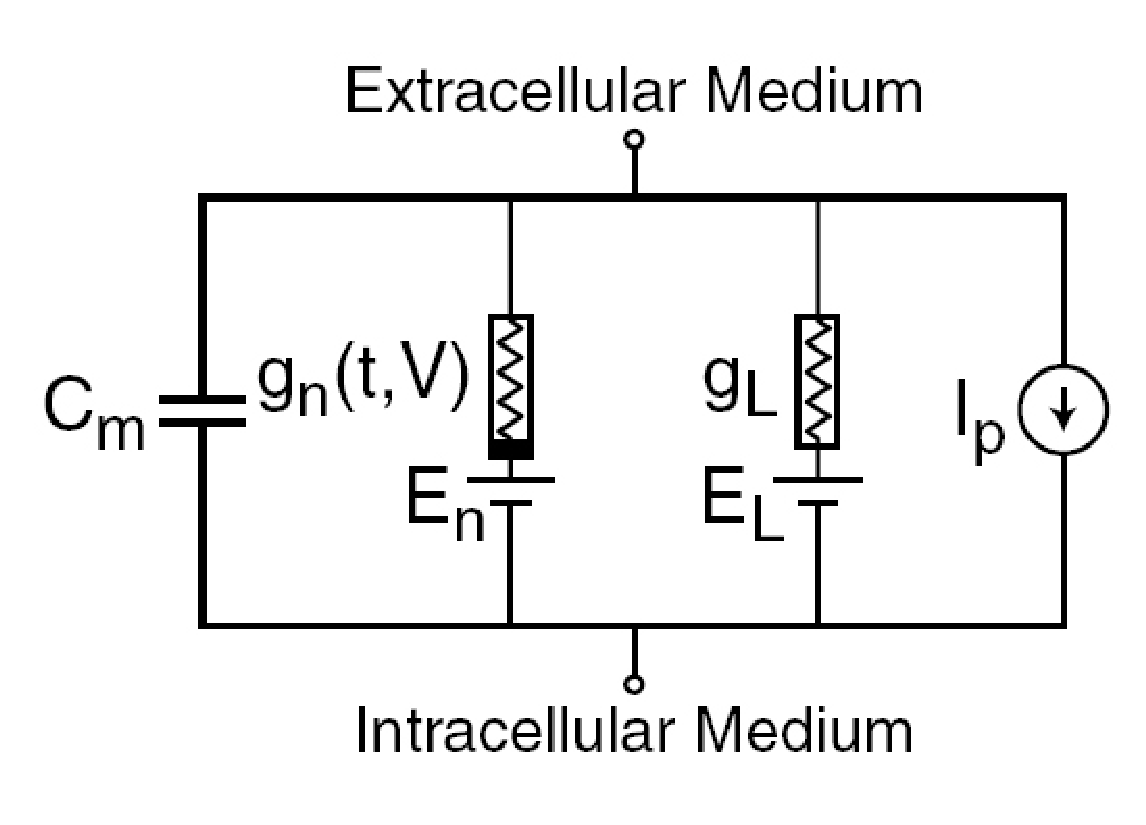
\includegraphics[height=4cm]{./images/Hodgkin-Huxley.eps}}
\caption{Hodgkin-Huxley model for cell membrane}\label{fig:Hodgkin-Huxley}
\end{figure}

Fig.\ref{fig:Hodgkin-Huxley} is explained as follows
\begin{enumerate}
  \item The lipid bilayer functions as an electrical insulator and is
  represented as a capacitor ($\Csc$ [Faraday per unit area]). 

  \item Leak current: with passive linear ($g_L$) conductances
  
\begin{equation}
I_L = g_L (V_m - E_L)
\end{equation}
  
  leak channels account for natural permeability of membrane and
  is considered constant
  
  \item Voltage-gated currents: the current caused by the gating of $V_m$-gated
  ion channels with conductance ($g_n$).
\begin{equation}
I_n = g_n (V_m - E_n)
\end{equation}
with $g_n(t,v_m)$ can be a non-linear function of $V_m$.

%   The electrochemical gradients driving the flow of ions are represented by
%   batteries (E), 
  
  \item Ion pumps and exchangers are represented by current sources (Ip).

 sodium-potassium and sodium-calcium bumps are the best known.
  
\end{enumerate}

In the integrate-and-fire neuron model the state of the neuron is characterized
by its membrane potential $V_m(t)$. 
% The neuron (indeed the soma) is modelled as 
% a sphereical shell, i.e. a 'leaky integrator' of its input
% $I(t)$:
% \begin{equation}
% \tau_m \frac{dV}{dt} = 	-V(t) + R_m.I_s(t) + R_m. I_\app(t)
% \label{eq:leaky_integrator}
% \end{equation}
% with $V(t)$ is the membrane potential at time $t$, $\tau_m$ is the membrane time
% constant and $R_m$ is the membrane resistance. Here, the current is leaky via
% the membrane which is modelled as a capacitor in parallel with a resistance
% $R_m$. The equivalent form is 
% \begin{equation}
% C \frac{dV}{dt} = I_\leak(t) + I_s(t) + I_\app(t)
% \end{equation}
% with $I_\leak(t)$ is the current due to passive leak across the membrane.

\begin{equation}
\tau_m \frac{dV_m}{dt} = 	R_m.I_s(t) + R_m. I_\app(t) + R_m. I_\leak(t) 
\label{eq:leaky_integrator}
\end{equation}
or
\begin{equation}
\Cm \frac{dV_m}{dt} = I_s  + I_\app + I_\leak
\end{equation}
which is the summation of
\begin{itemize}
  \item leaky current $I_\leak$: Sect.\ref{sec:leaky-current}

  \item synaptic inputs $I_s$: Sect.\ref{sec:synaptic-input}

  
  \item injected current $I_\app$ (rectangular current pulse)

As $i_\app$ (mA) is injected at the center, Fig.\ref{fig:sphere_cell}.
Then, the current density is
\begin{eqnarray}
  \label{eq:4071}
  I_\app = \frac{i_\app}{4\pi a^2}
\end{eqnarray}
with $a$ is the radius of the sphere (cm) and the unit of $I_\app$ is
currents per unit surface area (mA/cm$^2$ or mA/mm$^2$).

\end{itemize}

% \subsection{Electrotonus behavior (i.e. subthreshold condition)}
% \label{sec:electrotonus-behavior}


\subsection{ * Leaky current}
\label{sec:leaky-current}

Under subthreshold condition (Sect.\ref{sec:electrotonus_linearbehavior}), i.e.
the membrane resistivity $R_m$ is a constant and is independent from the
membrane voltage $V$ (mV). This is true when the voltage $V_m$ is subthreshold
(Sect.\ref{sec:electrotonus_vs_transient}).

Then, the leaky current {\bf leaky} represents the decay with a characteristic
time constant $\tau_m$ (the membrane time constant). 
\begin{equation}
I_\leak = - \frac{\Cm}{\tau_m}\left( V_m - E_\rest \right)
\end{equation}
with $\tau_m$ is the passive membrane time constant
(Sect.\ref{sec:membr-time-const-1}).

Then, the temporal change of the
subthreshold transmembrane potential is given
\begin{eqnarray}
  \label{eq:494}
  v = i_\app R(1-e^{-t/\tau})
  % V = I_\app R(1-e^{t/\tau})
\end{eqnarray}
with $\tau_m=\Rm\Csc=\R\C$ is the membrane time constant.  Thus, the
threshold voltage $v_s=i_\app R$ is the steady-state value when
$t\rightarrow \infty$.

  

\subsection{ * Synaptic inputs}
\label{sec:synaptic-input}

The synaptic input can be excitatory or inhibitory and comes from many synapses.
These inputs are each weighted by the respective synaptic strength which is
modeled as a weight term $w_i$
(Sect.\ref{sec:leaky-integrate-and-fire-weight-parameters}) at each synapse $i$.

\begin{equation}
I_s(t) = \sum_k \EPSC_k \times w_k + \sum_j \IPSC_j \times w_j
\end{equation}

The spike firing at the presynaptic neuron $k$ at time $t^{(f)}_k$ (NOTE:
$t^{(f)}$=firing time) on neuron $y$ generates an excitatory 
postsynaptic current pulse $\EPSC_{yk} \times w_{yk}$; similarly at presynaptic
neuron $k$ on neuron $y$ generates an inhibitory postsynaptic current
$\IPSC_{yj} \times w_{yj}$. Here, we can ignore the subscript $y$ as we consider
as the signal projected on the current neuron.


The question is how we want to model $\EPSC$ (or $\IPSC$)?
\begin{itemize}
  \item as a current injection (current synapse)
  
  \item as a change in conductance (conductance synapse)
  
\begin{equation}
\begin{split}
\EPSC = g(t-t^{(f)}_j) \times (V_m - E_\syn) \\
\IPSC = g(t-t^{(f)}_j) \times (V_m - E_\syn)
\end{split}
\end{equation}  
so for a neuron $y$
\begin{equation}
I_s(t,y) = \sum_k \EPSC_k \times w_k + \sum_j \IPSC_j \times w_j
\end{equation}
\end{itemize}
\textcolor{red}{Synaptic input is more accurately modeled as a change in
conductance, rather than modeled as a current injection}

% \begin{equation}
% I_s(t) = \sum_i \IPSC_i \times w_i
% \end{equation}
%  
Assume the neuron has $N_E, N_I$ number of excitatory synapses and inhibitory
synapses, respectively, Fig.\ref{fig:integrate-and-fire_neuron_synaptic-input}.
The synaptic input $I_s(t)$ can be modelled in two ways:
\begin{enumerate}
  \item current synapse (Sect.\ref{sec:synaptic-input-current}): $I_s(t) = f(a)$
  \item conductance synapse (Sect.\ref{sec:synaptic-input-conductance}): $I_s(t) = f(g)$
\end{enumerate}
  
Review: 
\begin{itemize}
  \item homogeneous synaptic input (i.e. pre-synaptic inputs come as a Poisson
  process constant rate):
  \citep{burkitt2006a}
  \item temporally inhomogeneous synaptic input (i.e. pre-synaptic inputs come
  as a Poisson process with dynamic rate and is a function of time):
  \citep{burkitt2006b}
\end{itemize}

%\section{Introduction}

% , are
% modeled either as injected current  (current synapse models in which
% summation is linear) or as a change in the membrane conductance (conductance
% synapse models in which summation of the synaptic input is nonlinear, i.e., the
% amplitude depends upon the value of the membrane potential)

%\subsection{RC leaky integrator (spherical cell)}
%\subsection{RC leaky integrator (model a soma)}

\subsection{ -- Current Synaptic input}
\label{sec:synaptic-input-current}

Current via all  synapses: $I_s(t)$
\begin{equation}
I_s(t) = \Cm \sum_{k=1}^{N_E} a_{E,k} S_{E,k}(t) + \Cm
\sum_{j=1}^{N_I}a_{I,j}S_{I,j}(t)
\end{equation}  
The amplitude $a_{E,k}>0$ and $a_{I,j}<0$ are the change in postsynaptic
potential due to a single synaptic event. 
The synaptic inputs $S_{E,k}(t)$ and
$S_{I,k}(t)$  can be modeled using one of the three below approaches

\subsection{ ---- delta function}
\textcolor{red}{\bf CASE 01} (synaptic inputs are Diract $\delta$ functions -
point current): the synaptic input causes a postsynaptic change in membrane
potential that is modeled with instantaneous rise and instantaneous decay. 

The pre-synaptic inputs $S_{E,k}(t)$ and $S_{I,k}(t)$ are linear sums of Dirac
functions 
\begin{equation}
\begin{split}
S_{E,k}(t) &= \sum_{t_{E,k}} \delta(t-t_{E,k}) \\
S_{I,j}(t) &= \sum_{t_{I,j}} \delta(t-t_{I,j}) \;\; k\ne j 
\end{split}
\end{equation} 
with $t_{E,k}$ is the time the excitatory event occur at synapse $k$, 
$t_{I,j}$ is the time the excitatory event occur at synapse $j$.

% The synaptic input $I_s(t)$ can be modelled in two ways:

\begin{figure}[htbp]
\centerline{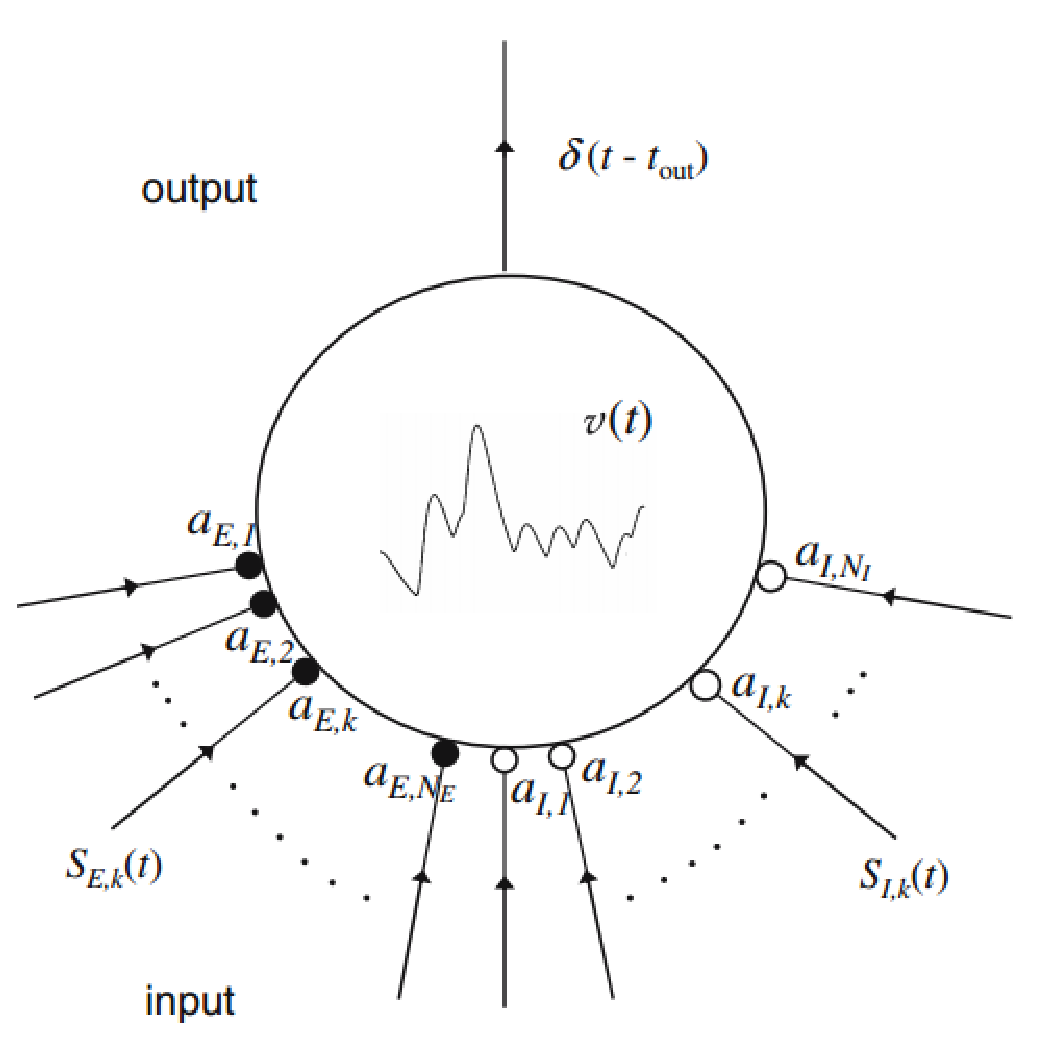
\includegraphics[height=6cm]{./images/integrate-and-fire_neuron_synaptic-input.eps}}
\caption{An
integrate-and-fire neuron
with $N_E$ excitatory
synapses and $N_I$
inhibitory synapses}\label{fig:integrate-and-fire_neuron_synaptic-input}
\end{figure} 


% The (normalized) postsynaptic response is a single $\delta$-function
% input of the neuron can be represented as 	
% \begin{equation}
% \varepsilon(t) = \frac{1}{\tau_m} e^{-t/\tau_m}\Theta(t)
% \end{equation}
% with  $\Theta(t)$ is the Heaviside step function to ensure causality in time.

% \subsection{ RC integrator + Synaptic input as current with finite time
% constant}

\subsection{ ---- exponentially decay function}
\textcolor{red}{\bf CASE 02} (synaptic inputs are exponential functions with
finite time constants): the synaptic input causes a postsynaptic change in
membrane potential that is model with instantaneous rise,
yet with an exponential decaying phase, with finite time constant $\tau_m$

The (normalized) postsynaptic response is
\begin{equation}
\varepsilon(t) = \frac{1}{\tau_m} e^{-t/\tau_m}\Theta(t)
\end{equation}
then
\begin{equation}
\begin{split}
I_{E,s} = \frac{a_E \Cm}{\tau_m} e^{-t/\tau_m} \Theta(t) \\
I_{I,s} = \frac{a_I \Cm}{\tau_m} e^{-t/\tau_m} \Theta(t)
\end{split}
\end{equation}
with $\tau_s$ is the synaptic input time constant. This time constant, in
general, different between different types of neurons; with  $\Theta(t)$ is the
Heaviside step function to ensure causality in time.

\subsection{ ---- alpha function}
\textcolor{red}{\bf CASE 03} (synaptic inputs are $\alpha-$ functions - alpha
function):
the synaptic input is modeled with a rising phase (a finite duration that is
believed to have strong effects on network dynamics)
\url{https://www.neuron.yale.edu/phpBB/viewtopic.php?f=15&t=2982}

Example (simple): input reaches the peak $\bar{g}_\syn$ at time $t-t_o=\tau$
\begin{equation}
g_\syn(t) = \bar{g}_\syn \frac{t-t_o}{\tau} e^{1-\frac{t-t_o}{\tau}}
\end{equation}
with a single time constant - the time course of the rise and decay are
correlated and cannot be separated. This function is not physiologically
realistic.

Example (more realistic): the input is the sum of 2 exponentials (one for rising
and one for decay phase) $\tau_\rise \ne \tau_\decay$.
The (normalized) postsynaptic response is now
\begin{equation}
\varepsilon(t) = \frac{e^{-t/\tau_\decay} - e^{-t/\tau_\rise}}{\tau_\decay - \tau_\rise} \Theta(t)
\end{equation} 


\begin{equation}
g_\syn(t) = \bar{g}_\syn f\left( e^{-(t-t_o)/\tau_\decay} -
e^{-(t-t_o)/\tau_\rise} \right)
\end{equation}
Here, the normalization factor $f(\cdot)$ ensures the peak amplitude is
$\bar{g}_\syn$; and the input reaches the peak at time
\begin{equation}
t_\peak = t_o + \frac{\tau_\decay \tau_\rise}{\tau_\decay - \tau_\rise} \ln
\left( \frac{\tau_\decay}{\tau_\rise} \right)
\end{equation}
and 
\begin{equation}
f = \frac{1}{e^{-(t-t_o)/\tau_\decay} -
e^{-(t-t_o)/\tau_\rise} }
\end{equation}
\begin{equation}
I_s \propto t.e^{-\alpha t}
\end{equation}
which can
be used to model the filtering effect of the dendritic tree upon
the voltage at the soma.

\subsection{ -- Conductance Synaptic input}
\label{sec:synaptic-input-conductance}

Current via all synapses
\begin{equation}
I_s(t) = \Cm [V_E - V(t)] \sum_{k=1}^{N_E} g_{E,k} S_{E,k}(t) + 
\Cm [V_E - V(t)] \sum_{k=1}^{N_I} g_{I,k}S_{I,k}(t)
\end{equation}  
The potential $V_E$ and $V_I$ are constants reversal potentials
($V_I \le V_\rest < V_\th < V_E$).

\url{http://homepages.inf.ed.ac.uk/mvanross/reprints/roth_mvr_chap.pdf}

\subsection{The weight $w_{ij}$}
\label{sec:leaky-integrate-and-fire-weight-parameters}

{\bf NOTE}: The abstract current variables $w_i$ (each is a linear equation)
are added to describe the variatey of firing patterns that neurons exhibit in
response to a step current; without this it cannot be reproduced. For a single
neuron, \textcolor{red}{the firing time} $t^{(f)}$ is the time when the
membrane potential $V_m$ of that neuron cross the threshold $V_\th$ from below,
i.e. $dVm/dt > 0$ and $V_m /ge V_\th$.

\begin{equation}
\tau_i \frac{dw_i} = a_i (V_m - E_\rev) - w_i 
\end{equation}

or (adaptation in the weight)
\begin{equation}
\tau_i \frac{dw_i} = a_i (V_m - E_\rev) - w_i + b_i \tau_i \sum_{t^{(f)}}
\delta(t-t^{(f)})
\end{equation}
with $b_i = 10$(pA) means that the adaptation current is 10 pA stronger after
the spike which serves as the 'jump' of the spike-triggered adaptation.

One possible biophysical interpretation of the increase is that during the
action potential calcium enters into the cell so that the amplitude of a
calcium-dependent potassium current is increased.


\subsection{Stochastic (intrinsic): randomness of neurotransmitter release +
channel gating}

As a point process, there is no channel gating or neurotransmitter release is
considered here. This is ignored in the model.

\subsection{Stochastic (external): randomness of synaptic input}

The external stochastic comes from the randomness of arrival time of synaptic
input. This is generally (indeed almost universally) modeled as a Poisson
process.

Although the input to a single synapse may differ significantly from a Poisson
process, so long as they can be assumed as a {\it renewal process}, i.e. the
successive interval time between two successive inputs (can be from the same
synapse of different synapse of the same type) are independent and identically
distributed, the combined input of a large number of synapses can be modeled as
a Poisson process, i.e. 
the sums of all pre-synaptic inputs on the current neuron are pooled Poisson
processes, one for excitatory and one for inhibitory inputs.
\begin{equation}
%\begin{split}
S_E(t) = \sum_k S_{E,k}(t) \quad S_I(t) = \sum_j S_{I,j}(t)
%\end{split}
\end{equation}
with spiking-rate $\lambda_E$ and $\lambda_I$, respectively
\citep{burkitt2006a}.

% The inputs are summed linearly and output spikes are represented as
% $\delta$-functions at the times when the membrane potential crosses threshold.
% \url{https://en.wikipedia.org/wiki/Dirac_delta_function}
% 
% with the occurrence of the input is modeled as a Poisson process with
% individual spiking rates $\gamma_{E,k}$ and $\gamma_{I,j}$, respectively.




\subsection{Numerical methods: LIF}

The original leaky integrate-and-fire model only the dynamics of $V_m$, not the
dynamics of any ion concentrations.
Also, the model only explicitly model the dynamics of $V_m$ at subthreshold
phase (Sect.\ref{sec:LIF-formula}). For transient phase, i.e. spike generation,
we can integrate the equation in
Sect.\ref{sec:leaky_integrate-and-fire_model-with-spike}.


$V_m$ is modeled using the formula
\begin{verbatim}
if v < Vthreshold: dVm/dt = I_ion + a - b*V_m

if v >= Vthreshold: v = c (reset) - keep this for a certain time, i.e. 
\end{verbatim}
with time-step $\Delta t = 1$ (ms).
\textcolor{red}{The integration takes 
only four  floating-point operations (additions, multiplications, etc.)} + one
comparison with the threshold.

The behavior it can exhibit with this model:
\begin{enumerate}
  \item Class I excitable (Sect.\ref{sec:Class-I-excitability})
  \item integrator (Sect.\ref{sec:coincidence-detectors})
\end{enumerate}

With only one variable, it cannot have phasic spiking, bursting of any  kind,
rebound  responses,  threshold  variability,  bistability of attractors, or
autonomous chaotic dynamic. Also, because of the fixed threshold, the spikes do
not have latencies.


INSPITE OF ITS OVER SIMPLIFICATION:
Focusing upon the subthreshold membrane properties and excluding the mechanisms
responsible for generating action potentials (i.e., the voltage-dependent sodium
and potassium channels) has proven to be a powerful tool in understanding the
information processing capabilities of neurons.
The model enabled Lapicque to calculate the spiking-rate of a neuron that was
coupled to a fixed-voltage stimulating electrode.
A more extensive analysis of Lapicque's model with injected current was carried
out by Hill (1936).



\section{Generalized linear integrate-and-fire model}

There are many properties of biological neurons that the leaky
integrate-and-fire model (Sect.\ref{sec:leaky_integrate-and-fire_model}) does
not reproduce.

\subsection{I\&F with adaptation: 2-D}

To model the slow-down in frequency of tonic spiking
(Sect.\ref{sec:tonic-spike-frequency-adapted}), a second ODE is added to emulate
the effect of outward $\K$ current, i.e. each firing increase the $\K$
activation gate $g$ via a Dirac delta function $\delta$. This outward current
slow down the 
\begin{verbatim}
dVm/dt = I_ion + a - b * V_m + g(d- V_m)
dg/dt = (delta(t) - g) / tau
\end{verbatim}

\textcolor{red}{By adding another parameter, each iteration requires
10 floating point operations.}

\subsection{I\&FB (fire-or-burst): 2-D}

Model thalamo-cortical neurons: The effect of the inactivation of the T-type
$\Ca$ current is added via $h$ gating, using Heaviside step function.

It takes between 9 and 13 operations per integration step.

\subsection{Spiking model: 2-D (Izhikevich 2003)}
\label{sec:Spiking-model}
\label{sec:Izhikevich-2003}

\citep{izhikevich2003} is also an abstract model, like integrate-and-fire, that
aims to produce spike trains. Unlike integrate-and-fire, the voltage changes
naturally to the peak value.

The model, based on bifurcation methodoligies, reduced the Hodgin-Huxley
neuronal model down to a 2-D system, i.e. two ODE equations, and has only one
nonlinear term $V_m^2$:

\begin{verbatim}
dVm/dt = 0.04 Vm^2 + 5 * Vm + 140 - u + I

du/dt = a * ( b * Vm - u) 
\end{verbatim}

which can be mapped to 3 ODEs linear system
\begin{verbatim}
Set: x = Vm^2

dx/dt = 2*Vm
dVm/dt = 0.04 * x + 5 * Vm + 140 - u + I
du/dt = a * ( b * Vm - u) 
\end{verbatim}

IMPORTANT: To make sure all spikes have the same magnitude, any value of $V_m > +30$ is
reset to +30mV, and then after the spike reaches its apex (+30mV), the membrane
voltage and the recovery variables are reset

\begin{verbatim}
if (Vm >= + 30 mV) then Vm <- c; u <- u + d
\end{verbatim}

NOTE: $a,b,c,d$ are dimensionless variables.
\begin{itemize}
  \item $a$ - describe the time-scale of the recovery variable $u$, i.e. smaller
  value of $a$ means slower recovery. He chosed $a=0.02$
  
  \item $b$ - describe the sensitivity of recovery variable $u$ to the
  subthreshold fluctuation of $V_m$. Greater value of $b$ means $u$ and $V_m$
  couple strongly resulting to possible subthreshold oscillations and
  low-threshold spiking dynamics.
  
He chose $b=0.2$.  The case b<a (b>a) corresponds to saddle-node (Andronov-Hopf)
bifurcation of the resting state.

  \item  $c$ - describes after-spike reset value caused by the fast
  high-threshold $\K$ conductances. 
  
  He chose $c = -65$ (mV).
  
  \item $d$ - describe after-spike reset value of $u$, caused by slow
  high-threshold Na+ and K+ conductances
  
  He chose $d=2$.
\end{itemize}

The new variable $u$ represents the membrane recovery variable, which which
accounts for the activation of $\K$ ionic currents and inactivation of $\Na$
ionic currents, and it provides negative feedback on $V_m$ (i.e. $(-u)$ term)

IMPORTANT: The part $0.04 V_m^2 + 140 + 5 V_m$ was chosen so that $V_m$ in the
scale of mV, and time has (milisecond) scale. NOTE: Other choices are also
available. The resting potential in the model is between
-70mV to -60mV depends on the value of $b$.

It  takes  only  13 floating  point  operations  to  simulate  1  ms  of  the 
model,  so  it  is  quite  ef ficient  in  large-scale  simulations  of 
cortical  networks.

 
\section{Nonlinear Integrate-and-Fire (RC+ Spike)}
\label{sec:Integrate-and-Fire-Spike}
\label{sec:leaky_integrate-and-fire_model-with-spike}

A spike (Sect.\ref{sec:spike}) is generated when the membrane potential
pass a threshold $V_\th$ (spiking threshold).
If the membrane potential does not pass this threshold, 
the potential eventually reset to the resting value via the
leaky process in eq.\ref{eq:leaky_integrator}.
% is recalculated with the initial value $V_r$.

\textcolor{red}{\bf CASE 01}: The spike, if occur, is represented as a
$\delta$-function, at the time the summation of all synaptic inputs to the given
neuron crosses the threshold.

\textcolor{red}{\bf CASE 02}: The spiking mechanism can be included in terms of
spiking current $I_\spike$ (Meffin et al. 2004)

\begin{equation}
I_\spike(t) = \Cm \left[ \frac{dV(t)}{dt} \right]^{-1}_{v=V_\th} (V_\reset -
V_\th) \delta[ V(t) - V_\th]
\end{equation}
with $\delta[\cdot]$ describes the Dirac delta function.


%action potential (spike) is 
% Instead, when $V(t)$
% reaches a certain threshold $V_\th$ (spiking threshold), 

% The neuron is injected with a current $I_\app(t)$, and the synaptic input to
% the neuron $I(t)$

\subsection{Quadratic integrate-and-fire (theta-neuron, Ermentrout-Kopell canonical model)}

The quadratic integrate-and-fire model provides some additional features to a
linear integrate-and-fire model: spike latency, bistability, and threshold
variability (which is Vthresh only when $I=0$).
\begin{verbatim}
dVm/dt = I + a (Vm - Vrest) (Vm - Vthresh); if Vm < Vpeak
Vm <- Vreset                              ; if Vm > Vpeak
\end{verbatim}

It takes only seven operation per integration step.
This should be the model of choice when one simulates large-scale networks of
integrators.

The  quadratic  I\&F  model  is  practically  as  efficient  as  the linear one,
and it exhibits many important properties of real neurons, such as spikes with
latencies, and bistability of resting and tonic spiking modes. However, it is
1-D (only $V_m$), and hence, it cannot burst and cannot exhibit spike frequency
adaptation.




\subsection{Exponential integrate-and-fire}

Synapses with exponentially decaying currents are used, only one timescale is
used.




\section{Spike response model (SRM0)}
\label{sec:spike-response-model}

The Spike Response Model (SRM) is a generalization of the leaky
integrate-and-fire model, just like Nonlinear Integrate-and-Fire model
(Sect.\ref{sec:Integrate-and-Fire-Spike}). However, instead of using
$I_\spike(t)$ which is a function of $V_m$, it uses 

 The motivation for the spike response model (SRM$_0$) lies in the
difficulty of finding analytic solutions of the diffusion-type
integrate-and-fire neuron models, especially when inhomogeneous
Poisson synaptic input is considered.

Here, the major difference is the reset potential after the threshold $V_\th$
is achieved by adding the $V_r$ an additional 'afterpotential' term
$\eta(t-t_f)$ (where $t_f$ is the time of firing the previous spike).
This term explicitly describes the time course of the action potential and the
afterpotential.
The leaky integrate-and-fire neuron model is a special case of the spike
response model, in which the afterpotential function $\eta(t)$ is a shot-noise
function
\begin{equation}
\eta(t) = (V_\reset - V_\th) e^{-(t-t_f)/\tau_m}\Theta(t-t_f)
\end{equation}

The spike response model also includes a dynamic threshold that is elevated
after a spike is generated.


\subsection{Stochastic model}

In general, there are two sources of noise associated with
the neural membrane potential:
\begin{enumerate}
  \item the 'noise' intrinsic to the neuron, i.e. the stochastic nature of the
  underlying mechanism control the release of neurotransmitter and the opening
  of channels
  
  \item the 'noise' from external factor, i.e. the  random arrival times
of the inputs
\end{enumerate}

The representation of the neuron as a point
(i.e., a single compartment) means that there is no clear distinction
between these two sources of noise, which can be
treated together in terms of the variance of the fluctuations in
the membrane potential.

They examined and concluded that the predominant source of randomness in the
model is the stochastic arrival times of the synaptic input, which is 
often modeled as a Poisson process.

IMPORTANT: \textcolor{red}{the inputs to a single synapse may differ significantly from a
Poisson process}.

In the spike
response model, the membrane potential explicitly depends
upon the time of the last spike. This time dependence enables
the refractory properties of the neuron to be modeled,
including a reduced responsiveness and increased threshold
after the generation of a spike, as well as a hyperpolarizing
spike-afterpotential.


